\documentclass[10pt]{article}
\usepackage[letterpaper]{geometry}
\geometry{verbose,tmargin=1in,bmargin=1in,lmargin=1in,rmargin=1in}
\usepackage{setspace}
\usepackage{ragged2e}
\usepackage{color}
\usepackage{titlesec}
\usepackage{graphicx}
\usepackage{float}
\usepackage{mathtools}
\usepackage{amsmath}
\usepackage[font=small,labelfont=bf,labelsep=period]{caption}
\usepackage[english]{babel}
\usepackage{indentfirst}
\usepackage{array}
\usepackage{makecell}
\usepackage[usenames,dvipsnames]{xcolor}
\usepackage{multirow}
\usepackage{tabularx}
\usepackage{arydshln}
\usepackage{caption}
\usepackage{subcaption}
\usepackage{xfrac}
\usepackage{etoolbox}
\usepackage{cite}
\usepackage{url}
\usepackage{dcolumn}
\usepackage{hyperref}
\usepackage{courier}
\usepackage{url}
\usepackage{esvect}
\usepackage{commath}
\usepackage{verbatim} % for block comments
\usepackage{enumitem}
\usepackage{hyperref} % for clickable table of contents
\usepackage{braket}
\usepackage{titlesec}
\usepackage{booktabs}
\usepackage{gensymb}
\usepackage{longtable}
\usepackage{listings}
\usepackage{cancel}
\usepackage{amsmath}
\usepackage[mathscr]{euscript}
\lstset{
    frame=single,
    breaklines=true,
    postbreak=\raisebox{0ex}[0ex][0ex]{\ensuremath{\color{red}\hookrightarrow\space}}
}

% for circled numbers
\usepackage{tikz}
\newcommand*\circled[1]{\tikz[baseline=(char.base)]{
            \node[shape=circle,draw,inner sep=2pt] (char) {#1};}}


\titleclass{\subsubsubsection}{straight}[\subsection]

% define new command for triple sub sections
\newcounter{subsubsubsection}[subsubsection]
\renewcommand\thesubsubsubsection{\thesubsubsection.\arabic{subsubsubsection}}
\renewcommand\theparagraph{\thesubsubsubsection.\arabic{paragraph}} % optional; useful if paragraphs are to be numbered

\titleformat{\subsubsubsection}
  {\normalfont\normalsize\bfseries}{\thesubsubsubsection}{1em}{}
\titlespacing*{\subsubsubsection}
{0pt}{3.25ex plus 1ex minus .2ex}{1.5ex plus .2ex}

\makeatletter
\renewcommand\paragraph{\@startsection{paragraph}{5}{\z@}%
  {3.25ex \@plus1ex \@minus.2ex}%
  {-1em}%
  {\normalfont\normalsize\bfseries}}
\renewcommand\subparagraph{\@startsection{subparagraph}{6}{\parindent}%
  {3.25ex \@plus1ex \@minus .2ex}%
  {-1em}%
  {\normalfont\normalsize\bfseries}}
\def\toclevel@subsubsubsection{4}
\def\toclevel@paragraph{5}
\def\toclevel@paragraph{6}
\def\l@subsubsubsection{\@dottedtocline{4}{7em}{4em}}
\def\l@paragraph{\@dottedtocline{5}{10em}{5em}}
\def\l@subparagraph{\@dottedtocline{6}{14em}{6em}}
\makeatother

\newcommand{\volume}{\mathop{\ooalign{\hfil$V$\hfil\cr\kern0.08em--\hfil\cr}}\nolimits}

\setcounter{secnumdepth}{4}
\setcounter{tocdepth}{4}
\begin{document}

\title{ME 280a: HW 5}
\author{April Novak}

\maketitle

\section{Introduction and Objectives}

The purpose of this study is to describe in great detail the process to solve a 3-D elastics problem, and also to generate a 3-D mesh with the appropriate connectivity matrix to be used for placing the local matrices and vectors into the global matrices and vectors.

\section{Procedure}
\label{sec:Procedure}

This section details the problem statement and mathematical method used for solving the problem.

\subsection{Theoretical Problem Statement}

The theory of elasticity is based on the continuum approximation, which assumes that the length scale on which solid particles exchange momentum is much smaller than the length scale characterizing the problem. An Eulerian perspective is adopted in the derivation of the governing equations, since control-volume-based approaches are much more amenable to solution than Lagrangian approaches. The deformation gradient tensor \(\bar{\bar{F}}\) is used to map between two different coordinate systems. One of these coordinates frames is defined by the coordinates \(x_i\) (the present coordinates), and the other by \(X_i\) (the reference coordinates):

\begin{equation}
\label{eq:DeformationGradient}
F_{ij}\equiv\frac{\partial x_i}{\partial X_i}
\end{equation}

The Jacobian \(\mathscr{J}\) is defined as the determinant of the deformation gradient tensor, and is required to transform integrals over the physical domain to the master element for application of quadrature rules:

\begin{equation}
\mathscr{J}\equiv \det{\bar{\bar{F}}}
\end{equation}

To have a physically meaningful transformation between two coordinate frames, the Jacobian must be positive. A balance of linear momentum in an arbitrary continuum is:

\begin{equation}
\label{eq:Cauchy}
\frac{d}{dt}\int_{\Omega}\rho\dot{\textbf{u}}dV=\int_{\partial\Omega}\vv{t}dS+\int_{\Omega}\rho\textbf{b}dV
\end{equation}

where \(\Omega\) is the domain of the continuum (a volume), \(rho\) is the density, \(\textbf{u}\) is the displacement vector, \(\partial\Omega\) represents the boundary of the volume domain (a surface \(S\)), \(\vv{t}\) represents the traction (loading on a surface), and \(\vv{b}\) represents a body force such as gravity. Eq. \eqref{eq:Cauchy} is no more than the Cauchy balance of linear momentum. By the Cauchy theorem, where surface forces are balanced on a tetrahedron, the traction is equivalent to:

\begin{equation}
\label{eq:Traction}
\vv{t}\equiv\bar{\bar{\sigma}}^T\cdot\hat{n}
\end{equation}

where \(\hat{n}\) is a unit normal and \(\bar{\bar{\sigma}}\) is the stress tensor, with components \(\sigma_{ji}\), where \(j\) refers to the face on which the stress acts, and \(i\) the direction in which the stress points. The transpose appears in the above equation because, in fluids scenarios, the stress is usually defined in the opposite manner such that the first index refers to the direction in which the stress points, and the second index the face on which the stress acts.

The stress tensor is symmetric in virtually all fluids applications, and in applications for which there are no ``micro-stresses'' in the body. In other words, from a balance of angular momentum, and by inserting the Cauchy balance of momentum in Eq. \eqref{eq:Cauchy}, the stress tensor is symmetric. Because the Cauchy balance of momentum was used, it was inherently assumed that the only moments on the body were due to the forces on the body, and hence this conclusion is consistent with that in the text.

Inserting Eq. \eqref{eq:Traction} into Eq. \eqref{eq:Cauchy}:

\begin{equation}
\label{eq:Cauchy2}
\frac{d}{dt}\int_{\Omega}\rho\dot{\textbf{u}}dV=\int_{\partial\Omega}\bar{\bar{\sigma}}^T\cdot\hat{n}dS+\int_{\Omega}\rho\textbf{b}dV
\end{equation}

If mass is conserved in this continuum (it is assumed so), then the material derivative on the LHS of the above equation can be moved inside the integration to act only on \(\cdot{\textbf{u}}\). This can conceptually be understood if the integral is divided into a finite sum over material elements. In a material element, mass is assumed conserved such that the time rate of change of \(\rho dV\) is zero, which is why the time derivative acts only on \(\cdot{\textbf{u}}\) (This also assumes that the coordinate system is not moving in time).

\begin{equation}
\label{eq:Cauchy3}
\int_{\Omega}\rho\ddot{\textbf{u}}dV=\int_{\partial\Omega}\bar{\bar{\sigma}}^T\cdot\hat{n}dS+\int_{\Omega}\rho\textbf{b}dV
\end{equation}

Applying Gauss's divergence theorem, which implicitly assumes that \(\bar{\bar{\sigma}}\) is sufficiently smooth, and dropping the transpose on the stress tensor with the assumption that it is symmetric:

\begin{equation}
\label{eq:Cauchy4}
\int_{\Omega}\rho\ddot{\textbf{u}}dV=\int_{\Omega}\nabla\cdot\bar{\bar{\sigma}}dV+\int_{\Omega}\rho\textbf{b}dV
\end{equation}

Then, by rearranging:

\begin{equation}
\label{eq:Cauchy5}
\int_{\Omega}\left(\rho\ddot{\textbf{u}}-\nabla\cdot\bar{\bar{\sigma}}-\rho\textbf{b}\right)dV=0
\end{equation}

Because the selection of the control volume was arbitrary, the integrand must equal zero:

\begin{equation}
\label{eq:Cauchy6}
\rho\ddot{\textbf{u}}=\nabla\cdot\bar{\bar{\sigma}}+\rho\textbf{b}
\end{equation}

Eq. \eqref{eq:Cauchy6} represents a balance of linear momentum, and is very general. It applies equally to fluids and solids, until a constitutive relationship is introduced for \(\bar{\bar{\sigma}}\). The theory of linear elasticity is now introduced in order to provide the constitutive relationship for \(\bar{\bar{\sigma}}\). 

From the definition of the deformation gradient tensor \(\bar{\bar{F}}\) in Eq. \eqref{eq:DeformationGradient}, the Lagrangian strain tensor \(\textbf{E}\) is defined as:

\begin{equation}
\textbf{E}\equiv\frac{1}{2}\left(\nabla_X\textbf{u}+(\nabla_X\textbf{u})^T+\underbrace{(\nabla_X\textbf{u})^T\cdot\nabla_x\textbf{u}}_\text{higher-order term}\right)
\end{equation}

where \(\nabla_X\) indicates a gradient with respect to the reference coordinate \(X\). With the linear theory of elasticity, deformations are assumed to be small such that the higher order term above can be neglected. The infinitesimal strain \(\textbf{e}\) is defined as:

\begin{equation}
\textbf{e}\equiv\frac{1}{2}\left(\nabla\textbf{u}+(\nabla \textbf{u})^T\right)
\end{equation}

and for small deformations, \(\textbf{E}\approx\textbf{e}\). (I couldn't figure out how to get the ``epsilon'' variable to work out, so epsilon is replaced by \(e\) in this document). The argument of the gradient has been dropped for simplicity. A similar derivation of a conservation of energy equation gives:

\begin{equation}
\rho\dot{w}=\bar{\bar{\sigma}}:\nabla\dot{\textbf{u}}-\nabla\cdot\textbf{q}+\rho z
\end{equation}

where \(w\) is the internal energy per unit mass, \(\textbf{q}\) the heat flux vector, and \(z\) the volumetric heating source. If thermal effects are neglected, then the above equation simplifies to:

\begin{equation}
\rho\dot{w}=\bar{\bar{\sigma}}:\nabla\dot{\textbf{u}}
\end{equation}

Applying the chain rule to the LHS above:

\begin{equation}
\rho\frac{\partial w}{\partial \textbf{e}}:\frac{d\textbf{e}}{dt}=\bar{\bar{\sigma}}:\nabla\dot{\textbf{u}}
\end{equation}

from which it is clear that:

\begin{equation}
\label{eq:StressDef}
\bar{\bar{\sigma}}=\rho\frac{\partial w}{\partial\textbf{e}}
\end{equation}

In order to develop a constitutive relationship for the theory of linear elasticity, it is assumed that a stored elastic energy function exists that depends only on the deformation. For small strains beginning from an undeformed state, energy is stored in the material. The stored elastic energy function \(W\) is by definition:

\begin{equation}
W\equiv \rho w
\end{equation}

The simplest function that satisfies Eq. \eqref{eq:StressDef} is:

\begin{equation}
W=\frac{1}{2}\textbf{e}:\textbf{IE}:\textbf{e}
\end{equation}

where \(\textbf{IE}\) is the fourth rank elasticity tensor. With these assumptions, the constitutive relationship for the stress tensor becomes:

\begin{equation}
\label{eq:1}
\bar{\bar{\sigma}}=\textbf{IE}:\textbf{e}
\end{equation}

Due to the linear relationship between stress and strain, this constitutive relationship is referred to as the ``theory of linear elasticity.'' Because \(\textbf{IE}\) is a fourth-order tensor, it has 81 unique entries (\(3^4=81\)). However, because the stress tensor is symmetric, there are actually only 36 unique entries. Because \(W\) is a scalar, \(\textbf{IE}\) must be symmetric, which implies that \(\textbf{IE}^T=\textbf{IE}\). Hence, the 36 unique constants reduce to 21. With all 36 constants, the relationship in Eq. \eqref{eq:1} is:

\begin{equation}
\begin{bmatrix}\sigma_{11} \\ \sigma_{22} \\ \sigma_{33} \\ \sigma_{12} \\ \sigma_{23} \\ \sigma_{31}\end{bmatrix}=
\begin{bmatrix}E_{1111} & E_{1122} & E_{1133} & E_{1112} & E_{1123} & E_{1113} \\
E_{2211} & E_{2222} & E_{2233} & E_{2212} & E_{2223} & E_{2213} \\
E_{3311} & E_{3322} & E_{3333} & E_{3312} & E_{3323} & E_{3313}\\
E_{1211} & E_{1222} & E_{1233} & E_{1212} & E_{1223} & E_{1213}\\
E_{2311} & E_{2322} & E_{2333} & E_{2312} & E_{2323} & E_{2313}\\
E_{1311} & E_{1322} & E_{1333} & E_{1312} & E_{1323} & E_{1313}\\
\end{bmatrix}
\begin{bmatrix}e_{11} \\ e_{22} \\ e_{33} \\ 2e_{12} \\ 2e_{23} \\ 2e_{31}\\
\end{bmatrix}
\end{equation}

where the strain vector shows that \(e_{12}=e_{21}\). For isotropic materials, \(\textbf{IE}\) simplifies by defining two parameters, \(\kappa\) and \(\mu\):

\begin{equation}
\textbf{IE}=\begin{bmatrix}\kappa+\frac{4}{3}\mu & \kappa-\frac{2}{3}\mu & \kappa-\frac{2}{3}\mu & 0 & 0 & 0\\
\kappa-\frac{2}{3}\mu & \kappa+\frac{4}{3}\mu & \kappa-\frac{2}{3}\mu & 0 & 0 & 0\\
\kappa-\frac{2}{3}\mu & \kappa-\frac{2}{3}\mu & \kappa+\frac{4}{3}\mu & 0 & 0 & 0\\
0 & 0 & 0 & \mu & 0 & 0\\
0 & 0 & 0 & 0 & \mu & 0\\
0 & 0 & 0 & 0 & 0 & \mu\\
\end{bmatrix}
\end{equation}

The eigenvalues of \(\textbf{IE}\) are directly proportional to \(\mu\) and \(\kappa\), and hence both \(\mu\) and \(\kappa\) must be positive in order to retain the positive definiteness of \(\textbf{IE}\). Combining the above results with the conservation of momentum statement in Eq. \eqref{eq:Cauchy6}, the balance of momentum for a linear elastic system is:

\begin{equation}
\label{eq:Cauchy7}
\rho\ddot{\textbf{u}}=\nabla\cdot(\textbf{IE}:\nabla \textbf{u})+\rho\textbf{b}
\end{equation}

where recall that \(\textbf{u}\) is the vector-valued displacement. The finite element implementation, beginning with the weak form, is discussed next.

\subsection{Finite Element Implementation}

\subsubsection{The Weak Form}

The weak form of Eq. \eqref{eq:Cauchy7} is obtained by multiplying through by a test function \(\textbf{v}\), where, like \(\textbf{u}\), \(\textbf{v}\) is a vector-valued function. Then, integrating over the body:

\begin{equation}
\int_{\Omega}\rho\ddot{\textbf{u}}\cdot \textbf{v}d\Omega=\int_{\Omega}\nabla\cdot(\textbf{IE}:\nabla \textbf{u})\cdot\textbf{v}d\Omega+\int_{\Omega}\rho\textbf{b}\cdot\textbf{v}d\Omega
\end{equation}


\subsection{Mesh Generator}

This section discusses the mesh generator used to mesh the tubular ``S'' structure given in the assignment. The meshing begins in each \(\theta\)-chunk. For the circular cross-section structure, the \(x\) and \(y\) coordinates are related to each other by:

\begin{equation}
\label{eq:xy}
x^2+y^2=r
\end{equation}

where \(r\) is the inner radius of the tubular structure. Each piece in the circumferential direction is defined according to \(\theta\), where \(0\leq\theta\leq2\pi\) defines the ``slice'' parallel to \(\vv{e}_r\). The generation of the mesh is based on determining the coordinates of each node. The first node is assigned to the first ``slice'' for \(\theta=0\). In the discussion of the mesh generator, ``slice'' refers to each plane for which there exists a hollowed annulus (that is meshed according to the number of layers and circumferential points). \(\Theta\) is the angle referring to the circumferential angle, while \(\theta\) refers to the angle in each slice. The overall algorithm for generating the coordinates for the mesh is as follows:

\begin{enumerate}
\item Begin with slice for \(\Theta=0\). Beginning then for \(\theta=0\), move counterclockwise around the first layer (inner surface of the tube). Increment \(\theta\) in units of \(2\pi/N_c\), and for each \(\theta\), assign the \(x\) and \(y\) coordinates according to Eq. \eqref{eq:xy}. 
\item After finishing the inner layer, increase \(r\) by \(dt\), where \(dt\) is the thickness of each layer, to move to the next layer, then repeat step 1. 
\item Repeat steps 1 and 2 until all layers in each slice have been meshed, where for each layer, \(dt\) is added. 
\item Now that a slice has been meshed, repeat for all slices. This requires determining the \(x,y,z\) centers for each new slice. This is performed by sweeping through \(\Theta\). The \(y\) coordinate is \(y=0\) for all points, while the \(x\) coordinate continually increases moving from slice to slice, and the \(z\) coordinate is positive for the left half of the tube, and negative for the right half of the tube. 
\item Now that all slices have been meshed, the mesh looks like as follows for \(N_c=8, N_\theta=8, N_t=3\). 

\begin{figure}[H]
  \centering
  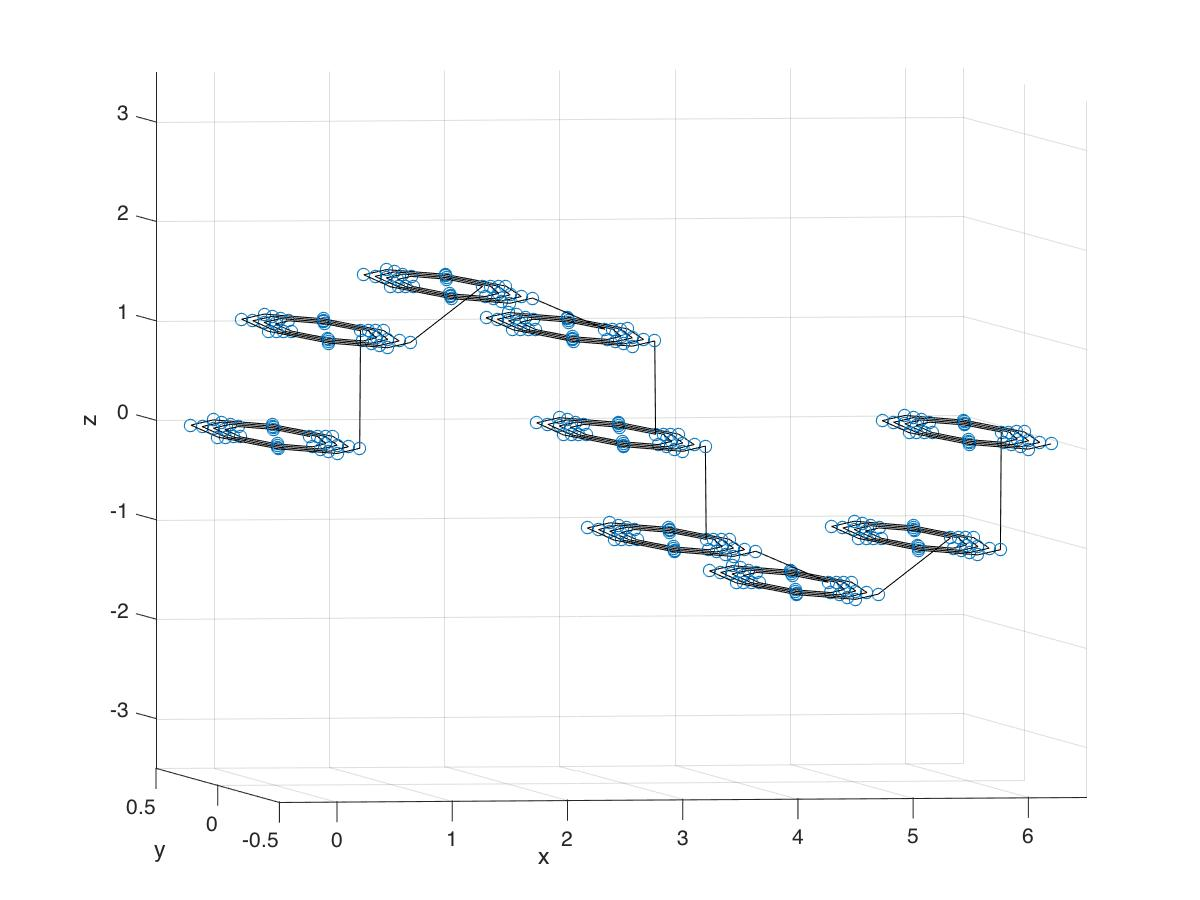
\includegraphics[width=10cm]{NoTilt.jpg}
  \caption{Mesh for \(N_c=8, N_\theta=8, N_t=3\) with no tilt to the slices. Lines connect each coordinate for better visuality.}
\end{figure}

The next step is to rotate the slices appropriately through the angle \(\Theta\) for each slice so that a tubular structure is formed. Only the \(x\) and \(z\) coordinates must be modified. To perform the tilt, the following quantities are computed using trigonometry:

\begin{equation}
\begin{aligned}
w=\sin{(\pi/2-\Theta)}(r+dt)\cos{(\theta)}/\sin{(pi/2)}\\
h = w\sin{(\Theta)}\\
p = w\cos{(\Theta)}\\
\end{aligned}
\end{equation}

To tilt the z-coordinate, for points in the first and fourth quadrant of each slice:

\begin{equation}
z_{new} = z - (-1)^{tube}h
\end{equation}

And for points in the second and third quadrant of each slice:

\begin{equation}
z_{new} = z + (-1)^{tube}h
\end{equation}

where \(tube\) is a variable indicating whether or not the slice is in the left or right half of the tube. For the left half of the tube, \(tube=1\), and in the right half, \(tube=2\).

\item Then, tilt the x-coordinates. For points in the first and fourth quadrants of each slice:

\begin{equation}
x_{new} = x + p
\end{equation}

And for points in the second and third quadrants of each slice:

\begin{equation}
x_{new} = x - p
\end{equation}

\item Finally, tilt the slices that exactly align with the peak and valley of the tube (for odd numbers of \(N_\theta\), this would not be performed). For the slices that align with the peaks and for nodes in the first and fourth quadrants, adjust the \(z\) coordinates according to:

\begin{equation}
z_{new} = z - (r+dt)\cos{(\theta)}
\end{equation}

And for points in the second and third quadrants:

\begin{equation}
z_{new} = z + (r+dt)\cos{(\theta)}
\end{equation}

The \(x\)-coordinates are adjusted by simply setting all of them to the centroid coordinate for that slice. 
\end{enumerate}

This process is fairly complicated, and reveals why meshing software is so valuable. The process here is left fairly general that it can apply for any values of \(N_\theta, N_c, N_t\), but any slight change in the geometry completely invalidates the program. The final mesh for \(N_c=8, N_\theta=8, N_t=3\) is shown below. This mesh is shown because the requested mesh with only \(N_c=4\) is relatively difficult to perceive in a 3-D plot in Matlab, so the following plot better reveals the mesh. Lines are drawn between each coordinate.

\begin{figure}[H]
  \centering
  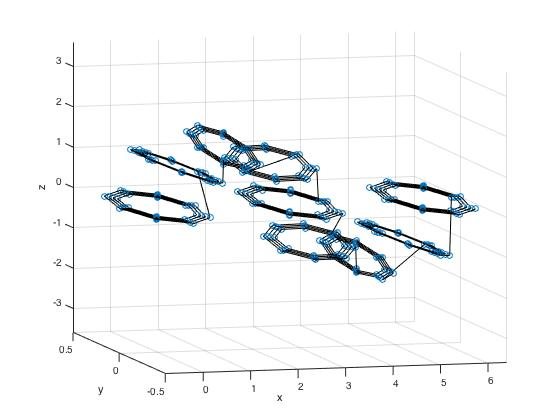
\includegraphics[width=10cm]{RefinedMesh.jpg}
  \caption{Mesh for \(N_c=8, N_\theta=8, N_t=3\). Lines connect each coordinate for better visuality.}
\end{figure}

The coarser mesh, for \(N_c=4, N_\theta=8, N_t=3\) is shown below, again with lines connecting each coordinate for better visibility.

\begin{figure}[H]
  \centering
  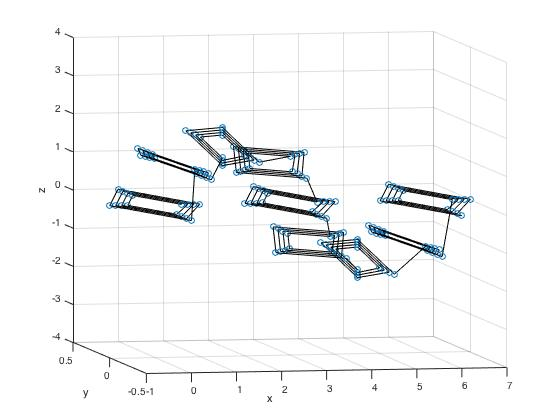
\includegraphics[width=10cm]{CoarseMesh.jpg}
  \caption{Mesh for \(N_c=4, N_\theta=8, N_t=3\). Lines connect each coordinate for better visuality.}
\label{fig:CoarseMesh}
\end{figure}

The mesh in Fig. \ref{fig:CoarseMesh} is shown below without the lines connecting each coordinate.

\begin{figure}[H]
  \centering
  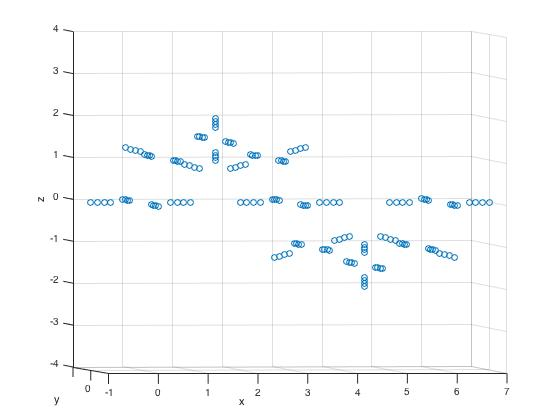
\includegraphics[width=10cm]{CoarseMeshNoLines.jpg}
  \caption{Mesh for \(N_c=4, N_\theta=8, N_t=3\).}
\end{figure}

Note that this assignment did not provide the dimensions of the tube, so I assumed that the inner radius of each arch was 1, the radius of the inner hole of the tube 0.3, and the thickness of the tube 0.2.

In order for this mesh to be useful for finite element implementation, a connectivity function must be defined to relate the local node numbering to the global node numbering. The mesh generated numbers the global nodes according to the order in which they were generated. For instance, the first 8 nodes are in the inner layer of the first slice, the next 8 are in the second layer of the first slice, and so on for the first slice. Then, moving to the next \(\Theta\) slice, the node numbering again begins on the inside of the tube and moves counterclockwise in layers until reaching the outside of the tube. This is shown schematically in the figures above by the black lines connecting the coordinates \textit{in the order in which the coordinates are generated}.

The connectivity matrix is an \(N\times4\) matrix, where \(N\) is the total number of elements and 4 is the number of local nodes per element (linear elements are assumed). 

\section{Appendix}

This section contains the complete code used in this assignment. 
\begin{comment}
\subsection{\texttt{FEProgram.m}}
This is the main code used for the problem solving.
\lstinputlisting[language=Matlab]{FEProgram.m}

\subsection{\texttt{BCnodes.m}}
This function applies boundary conditions.
\lstinputlisting[language=Matlab]{BCnodes.m}

\subsection{\texttt{condensation.m}}
This function separates out the matrix equation as in Eq. \eqref{eq:condensation}.
\lstinputlisting[language=Matlab]{condensation.m}

\subsection{\texttt{mesh.m}}
This function performs the meshing.
\lstinputlisting[language=Matlab]{mesh.m}

\subsection{\texttt{permutation.m}}
This function determines the permutation matrix for use with the connectivity matrix.
\lstinputlisting[language=Matlab]{permutation.m}

\subsection{\texttt{postprocess.m}}
This function postprocesses the FE solution and transforms it back to the physical domain using a linear system solve as described in Eq. \eqref{eq:LinearSolve}.
\lstinputlisting[language=Matlab]{postprocess.m}

\subsection{\texttt{quadrature.m}}
This function selects the quadrature rule.
\lstinputlisting[language=Matlab]{quadrature.m}

\subsection{\texttt{shapefunctions.m}}
This function contains the library of shape functions.
\lstinputlisting[language=Matlab]{shapefunctions.m}
\end{comment}
\end{document}